\part{Compte rendu du stage}

\section{Développement du script de base pour la sauvegarde et le chiffrement des données}

\subsection{Convention de l'ANSSI}

L'Agence Nationale de la Sécurité des Systèmes d'Information recommande l'utilisation de
l'algorithme de hachage \textbf{SHA-256} et l'usage de clé \textbf{RSA 2048 bits}.

\subsection{Consigne}

Le script de base devra être développé en \textit{Python 2.7} et devra remplir les conditions
suivantes :

\begin{enumerate}
     \item Indentation de 4 espaces, pas de tabulations.
     \item Deux répertoires : \textbf{src} et \textbf{dest}, le fichiers ne doivent pas être
     copiés de \textit{src} vers \textit{dest}, ce dernier répertoire ne devra contenir que du
     contenu chiffré.
     \item Calculer la somme SHA-256 des fichiers sources et l'afficher.
     \item Chiffrer les fichiers avec \textit{GnuPG} dans \textit{dest}.

     \begin{enumerate}
          \item Si le fichier n'existe pas, le créer.
          \item Si le fichier existe le nommer selon ce pattern : \textit{filename.X.gpg} où X
          varie de 1 à 5 (à la 6è itération, on supprime le fichier).
     \end{enumerate}

     \item Placer le code source dans un dépôt \textit{git}.
     \item Utiliser \textit{unittest} pour les tests unitaires.
\end{enumerate}

\subsection{Conclusion}

Cette partie du logiciel a été développée sous la forme d'un paquet \textit{Python}.

A l'aide d'un unique objet, on est capable de récupérer la liste des fichiers du répertoire
source, de calculer leurs sommes SHA-256 et de les chiffrer via \textit{GnuPG} :

\begin{verbatim}
from src.filemanager import FileManager

fm = FileManager.FileManager (srcpath, destpath)
filelist = fm.read_entries ()
checksum = fm.hash_entries (filelist)
fm.gpg_encrypt (filelist) # encrypt
\end{verbatim}

\section{Gestion de la base de données SQL}

La base de données SQL sera utilisée pour indexer les fichiers chiffrés sur l'espace de stockage.
Grâce à elle, on ne chiffrera pas plusieurs fois un même fichier, et on ne transférera pas sur
l'hôte distant plusieurs fois les mêmes données.

Il est donc impératif que la base de données contienne les informations suivantes :

\begin{description}
     \item[hash:] Le hash SHA-256 du fichier non chiffré, il sera utilisé en tant qu'index de la
               base de données SQL.
     \item[path:] Le chemin d'accès vers le fichier chiffré, ainsi pour un fichier chiffré on a le
               hash du fichier non chiffré qui y est associé.
     \item[sent:] La date à laquelle le fichier a été envoyé sur l'hôte distant (ou 0 s'il n'a pas
               été envoyé).
\end{description} ~

Voici par exemple ce que pourra contenir une table :

\noindent \begin{tabular}{| c | c | c |}
     \hline
     e3b0c44298fc1c149afbf4c8996fb92427ae41e4649b934ca495991b7852b855 & try/empty.gpg & 1320932458 \\ \hline
     fe19778cf1ce280658154f2b9c01ffbccd825a23460141dcf3794e7a2c0eb629 & oops.gpg & 1315472654 \\ \hline
     f2ca1bb6c7e907d06dafe4687e579fce76b37e4e93b7605022da52e6ccc26fd2 & test.gpg & 0 \\ \hline
\end{tabular} ~ \newline \newline

On aimerait cependant ne pas avoir à ce soucier du type de la base de données (\textit{MySQL}, \textit{SQLite},
...), il conviendra donc d'utiliser \textit{Django} pour la gestion de la base de données :

\begin{verbatim}
from django.db import models

class DatabaseEntry (models.Model):
     checksum = models.CharField (max_length = 64)
     path     = models.CharField (max_length = 256)
     sent     = models.DateTimeField ()
\end{verbatim}

\section{Intégration Django}

L'interface web étant également développé avec \textit{Django}, il convient donc d'intégrer notre script
dans une application \textit{Django} qui sera distribuée avec l'interface web.

Le projet, \textbf{delikatess}, se présente désormais sous la forme d'un projet \textit{Django} :

\begin{description}
     \item[webui:] L'interface web.
     \item[trackfile:] Le script de sauvegarde et de chiffrement.
     \item[sendit:] Le script d'envoie des fichiers chiffrés.
\end{description}

\subsection{trackfile}

L'application \textit{trackfile} est donc l'intégration de notre script à \textit{Django}.
Ainsi la base de données de notre script est commune à celle de \textit{Django} et de notre
future application web :

\begin{verbatim}
>>> from trackfile.utils import FileManager
>>> fm = FileManager (<gpg-key>, <source directory>, <destination directory>, nbackups = 7)
>>> fm.run ()
\end{verbatim}

\section{Intégration continue}

Afin de vérifier la validité du code source produit à chaque modifications, il va falloir développer
un script qui va devoir remplir les conditions suivantes :

\begin{itemize}
     \item Créer un environnement \textit{Python} virtuel (à l'aide de \textit{virtualenv} dans \textit{.venv}).
     \item Installer les dépendances du projet dans cet environnement (à l'aide du gestionnaire de paquets \textit{Python} : \textit{pip}).
     \item Exécuter les tests unitaires.
\end{itemize}

\begin{verbatim}
#!/bin/sh

echo "===> Creating virtual environment: .venv"
virtualenv .venv || exit 1

echo && echo && echo "===> Installing dependancies"
.venv/bin/pip install -r requirements.txt || exit 1

echo && echo && echo "===> Running test suite"
.venv/bin/python2.7 manage.py test || exit 1
\end{verbatim}

\section{Interface Web}

Maintenant que l'application \textit{trackfile} est terminée (pour le moment), le développement de l'application web
va pouvoir commencer. La création d'une nouvelle application \textit{Django} ne sera pas nécessaire, en effet, il ne
s'agit ici que d'une interface web. La base de donnée étant remplie par l'application \textit{trackfile}, notre interface
ne sera utilisée que pour en visualiser le contenu.

Notre projet \textit{Django} prend donc forme :

\begin{verbatim}
|-+ delikatess
| |-- __init__.py
| |-- manage.py
| |-- settings.py
| |-+ trackfile
| | |-- __init__.py
| | |-- models.py
| | |-- utils.py
| | |-- tests.py
| |-- urls.py
| |-- views.py
\end{verbatim}

Ici, le dossier \textit{trackfile} est celui de l'application, l'interface web ne sera contenue que dans le fichier
\textit{views.py}.

L'application web sera construite à l'aide du front-end \textit{Twitter Bootstrap}, de \textit{dajax} et \textit{dajaxice}
(plugins \textit{AJAX} pour \textit{Django}) :

\begin{description}
     \item[Twitter bootstrap :] \url{http://twitter.github.com/bootstrap}
     \item[dajaxice \& dajax :] \url{http://www.dajaxproject.com}
\end{description}


L'interface web se décomposera en différentes parties (cf. schéma I.2.2) :

\begin{itemize}
     \item Une barre d'outil (informera sur l'utilisateur connecté ainsi que le dossier courrant).
     \item Une vue en liste du contenu de l'espace de stockage.
     \item Une vue en arborescence dont les interactions sont couplées à la vue en liste.
     \item Un volet d'information sur le(s) fichier(s) sélectionné(s).
\end{itemize}

\subsection{La vue en arborescence}

La base de donnée peut être rapportée à une liste de chemin vers les fichiers chiffrés. Histoire
de hiérarchiser cela, à partir de cette liste, on génère un arbre (qui est donc stocké dans un
dictionnaire \textit{Python}, équivalent à du \textit{JSON}).

Ce \textit{JSON} est donc transmis à la template \textit{Django} qui s'occupera (à l'aide de \textit{jQuery})
de générer l'arborescence.

\begin{verbatim}
entries = DatabaseEntry.objects.all ()

# Create JSON tree
json = {"children": []}

for dbe in entries:
     folders = dbe.path.split (os.sep)
     d = json["children"]

     for name in folders:
          tmp = {}

          # Is it the end of the path ?
          if name == folders[-1]:
               tmp["name"] = str (name)
               tmp["hash"] = str (dbe.checksum)
               tmp["sent"] = dbe.sent
               d.append (tmp)
               break

          # Is it already in the tree ?
          alreadyin = False

          for child in d:
               if child["name"] == name:
                    alreadyin = True

                    # If already in, just go to the next level
                    if "children" in child:
                         d = child["children"]

                    break

          # If not already in, create it
          if alreadyin == False:
               tmp["name"] = str (name)
               tmp["children"] = []

               d.append (tmp)
               d = tmp["children"]
\end{verbatim}

Cet arbre \textit{JSON} est ensuite convertit en \textit{HTML} grâce à la librairie \textit{JavaScript} :
\textbf{PURE} (\url{http://beebole.com/pure/}), et avec un peu de \textit{JavaScript} supplémentaire, l'arbre
devient interactif.

\subsection{Le reste de l'interface}

Pour le reste de l'interface, tout se base sur cet arbre. Les deux autres éléments (la table et la barre du haut)
s'intègrent à ce dernier grâce à un peu de \textit{JavaScript} :

\begin{itemize}
     \item Un clic sur un dossier de l'arborescence provoque :

     \begin{itemize}
          \item L'apparition des sous-dossiers dans l'arborescence.
          \item La modification du chemin courant dans la barre du haut.
          \item Le chargement du contenu du dossier dans la table.
     \end{itemize}

     \item Un clic sur un éléments de la barre du haut provoque :

     \begin{itemize}
          \item L'apparition des sous-dossiers dans l'arborescence.
          \item La modification du chemin courant dans la barre du haut.
          \item Le chargement du contenu du dossier dans la table.
     \end{itemize}

     \item L'ouverture d'un dossier dans la table provoque :

     \begin{itemize}
          \item L'apparition des sous-dossiers dans l'arborescence.
          \item La modification du chemin courant dans la barre du haut.
          \item Le chargement du contenu du dossier dans la table.
     \end{itemize}
\end{itemize}

Comme on peut le voir, chaque action sur chaque élément de l'interface fait appel aux mêmes fonctions.

\section{Changement d'orientation du projet}

Jusque maintenant, le projet était une application unique mise en place chez le client.
Cette application comprenait le versionnage, le chiffrement, l'envoie des fichiers ainsi
que l'interface web.

L'hébergeur, montrant un certain intérêt pour le projet, a décidé d'héberger également
l'interface web. Le projet se présente donc de la manière suivante :

\begin{description}
     \item[Client:] Application de versionnage, de chiffrement et d'envoie des fichiers.
     \item[Hébergeur:] Application web.
\end{description}

Ainsi, il s'agit de développer un gestionnaire de version à notre sauce, j'entends par là :
indexer les fichiers, ne stocker que les différences, envoyer l'index et les fichiers sur un
serveur distant, ...

L'application web serait à ce logiciel ce qu'un \textbf{gitweb} est à \textit{git}.

\subsection{Architecture de l'application}

Lors d'une réunion, nous avons décidé d'organiser le projet de la manière suivante :

\begin{itemize}
     \item Les fichiers sont découpés en blocs de taille fixe.
     \item Chaque bloc est chiffré, puis compressé.
     \item Ce sont les blocs qui sont versionnés, ainsi que l'arborescence.
     \item Pour l'envoi et la réception des nouvelles versions, on développera une API.
     \item On n'utilise donc plus une base de données \textit{SQL} pour le versionnage, mais une base de données
     dans le système de fichiers.
     \item Pour la répartition des blocs sur le système de fichiers, on utilisera un serveur de \textbf{sharding}.
     \item Le tout reste développé en \textit{Python} et côté serveur on utilise toujours \textit{Django}.
\end{itemize}

Voici un schéma de l'architecture prévue :

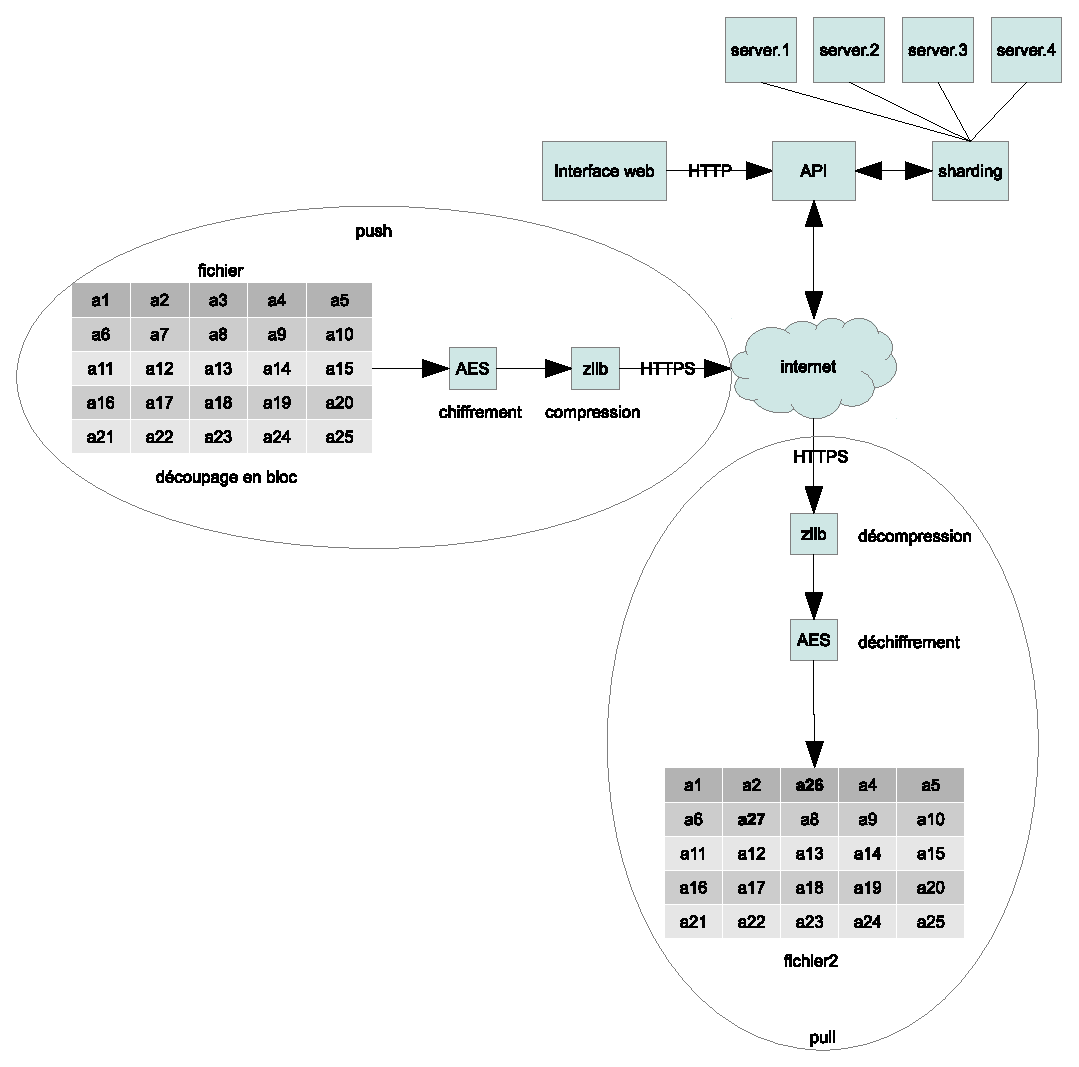
\includegraphics[scale=0.5]{img/schema.eps}

\subsection{Présentation de l'API}

L'API sera donc utilisée pour envoyer ou recevoir de nouvelles versions, voici un exemple de ce que pourrait être l'API :

\subsubsection{Réception d'une nouvelle version}

\begin{verbatim}
GET /v1/{id client}/HEAD
     On récupère les meta-données de la révision d'arborescence.
     <==  {'HEAD': {'{id rev}': ['aefd475c', 'efda58b8', '1d25aecb', '548ef9d2', 'effda55c']}}

POST /v1/{id client}/{id rev}/files
     On envoie la liste des fichiers inconnus de notre révision locale.
     ==>  {'files': ['aefd457c', '548ef9d2']}
     On récupère la liste des blocs de chaque fichiers.
     <==  {'files': {
               'aefd457c': ['efda85e6', '8426efca', '422eda43', '45227d7e',
                            '9436d5ef', 'eadcb5e8'],
               '548ef9d2': ['aef475de', 'eefab5bc'],
               'blocksize': '4k'
          }}

POST /v1/{id client}/{id rev}/blocks
     On envoie la liste des blocs inconnus.
     ==>  {'blocks': ['efda85e6', '422eda43', '45227d7e', 'eadcb5e8', 'eefab5bc']}
     On récupère l'URL de chaque bloc.
     <==  {'blocks': {
               'efda85e6': 'http://sharding1.static.9h37.fr/ef/da/efda85e6',
               '422eda43': 'http://sharding3.static.9h37.fr/42/2e/422eda43',
               '45227d7e': 'http://sharding1.static.9h37.fr/45/22/45227d7e',
               'eadcb5e8': 'http://sharding2.static.9h37.fr/ea/dc/eadcb5e8',
               'eefab5bc': 'http://sharding1.static.9h37.fr/ee/fa/eefab5bc'
     }}
\end{verbatim}

\subsubsection{Envoi d'une nouvelle version}

\begin{verbatim}
POST /v1/{id client}/HEAD
     On envoie notre révision locale actuelle de l'arborescence.
     ==>  {'HEAD': {'{id rev local}': ['aefd475c', 'efda58b8', '1d25aecb',
                    '548ef9d2', 'effda55c']}}
     On récupère l'identifiant de la nouvelle version allouée.
     <==  {'HEAD': '{id rev remote}'}

POST /v1/{id client}/{id rev remote}/files
     On envoie la liste des fichiers
     ==>  {'files': {
               'aefd457c': ['efda85e6', '8426efca', '422eda43', '45227d7e',
                            '9436d5ef', 'eadcb5e8'],
               '548ef9d2': ['aef475de', 'eefab5bc'],
               'blocksize': '4k'
          }}
     Le serveur nous envoie la liste des blocs inconnus.
     <==  {'blocks': ['efda85e6', '422eda43', '45227d7e', 'eadcb5e8', 'eefab5bc']}

FOREACH block in blocks
     PUT /v1/{id client}/{id rev remote}/blocks/{id block}
          {DATA}
\end{verbatim}
